\documentclass[10pt]{article}
\usepackage[a4paper,left=2cm,right=2cm,top=1.5cm,bottom=1.5cm]{geometry}
\usepackage[utf8]{inputenc}
\usepackage[T1]{fontenc}
\usepackage{amsmath}
\usepackage{amssymb}
\usepackage{graphicx}
\usepackage{abstract}
\usepackage{ctex}
\usepackage{mathtools}
\usepackage{amsxtra}
\usepackage[hidelinks]{hyperref}
%断词相关
\hyphenpenalty=5000
\tolerance=1000

\begin{document}
\tableofcontents
\section{什么是slam}
\numberwithin{equation}{section}

\textbf{运动方程}

机器人或者一个物体在空间中的运动都可以抽象为一个数学模型
\begin{align}\textbf{x}_k=f(\textbf{x}_{k-1},\textbf{u}_k,\textbf{w}_k) \end{align}
\indent 其中,$\textbf{u}_k$表示运动传感器的读书或者输入,$\textbf{w}_k$表示该过程中加入的噪声,$\textbf{x}_k$表示该时刻运
动物体所在位置,函数$f$描述这一个过程,即使不清楚这个过程的具体数学表达。

\textbf{观测方程}

与运动方程相对应的还有一个观测方程,它描述的是运动机器人在$textbf{x}_k$位置上观测到某些物体$\textbf{y}_k$产生的一个观测数据
$textbf{z}_{k,j}$,同样可以用一个抽象的函数$h$来表示这样一个关系:
\begin{align}\textbf{z}_{k,j}=h(\textbf{y}_i,\textbf{x}_k,\textbf{v}_{k,j})\end{align}
\indent 这里$\textbf{v}_{k,j}$是这一次的观测噪声。

上述两个方程描述了最基本的SLAM问题,当知道运动测量读书$u$,以及传感器的读书$z$时,如何求解定位问题(估计$\textbf{x}$)和建图问题
(估计$\textbf{y}$),这样就把SLAM问题建模成了一个状态估计问题:如何通过带有噪声的测量数据,估计内部的,隐藏着的状态变量。
\section{刚体的三维运动}
\numberwithin{equation}{section} %公式编号跟随章节
\textbf{内积}
\begin{align}\textbf{a} \cdot \textbf{b}=\textbf{a}^{T}\textbf{b}=\sum_{i=1}^{3}a_{i}b_{i}=|\textbf{a}||\textbf{b}|\cos<\textbf{a},
\textbf{b}>\end{align}

\textbf{外积}
\begin{align}\textbf{a}\times\textbf{b}=\left\|\begin{array}{lll}\textbf{e}_1 & \textbf{e}_2 & \textbf{e}_3 \\ a_1 & a_2 &
    a_3 \\ b_1 & b_2 & b_3 \end{array}\right\|=\left[\begin{array}{l}a_2b_3-a_3b_2 \\ a_3b_1-a_1b_3 \\ a_1b_2-a_2
        b_1\end{array}\right]=\left[\begin{array}{ccc}0 & -a_3 & a_2 \\ a_3 & 0 & -a_1 \\ -a_2 & a_1 & 0\end{array}
        \right]\textbf{b} \overset{def}{=}\textbf{a} \wedge \textbf{b}\end{align}

外积的结果是一个向量,它的方向垂直于这两个向量,大小为$|\textbf{a}||\textbf{b}|\sin<\textbf{a},\textbf{b}>$,是两个向量
张成的四边形的有向面积。

\textbf{旋转矩阵}

旋转矩阵各分量从定义推导上来看是两个坐标系基的内积,由于基向量的长度为1,所以实际上是各个基向量的夹角的余弦值,因此也称作\textbf{方向余弦矩阵}
,它实际上是一个行列式为1的正交矩阵。

对于n维旋转矩阵集合定义如下:
\begin{align}SO(n)=\{\textbf{R}\in \mathbb{R}^{n\times n} \textbf{R}\textbf{R}^{T}=\textbf{\emph{I}},det(\textbf{R})=1\}\end{align}

特别的$SO(3)$指三维空间的旋转,通过旋转矩阵就可以直接讨论两个坐标系之间的转换,而不用再从基开始谈起。

由于旋转矩阵为正交矩阵,它的逆(即转置)描述了一个相反的旋转,即$\textbf{R}^{-1},\textbf{R}^{T}$刻画来了一个与$\textbf{R}$相反的旋转矩阵。

对于两个坐标系1和坐标系2来说,向量$\textbf{a}$在两个坐标系下的坐标为$\textbf{a}_1,\textbf{a}_2$,它们之间的关系应该为:
\begin{align}\textbf{a}_1=\textbf{R}_{12}\textbf{a}_2+\textbf{t}_{12}\end{align}

这里的$\textbf{R}_{12}$是指把坐标系2的向量变换到坐标系1中,关于平移$\textbf{t}_{12}$,它实际意义上指的是坐标系1的原点指向坐标系2原点的向量。
注意在两个坐标系的相互变换中,其中的$\textbf{t}_{12}$和$\textbf{t}_{21}$并\textbf{不存在}$\textbf{t}_{12}=-\textbf{t}_{21}$这样的关
系,因为这两个坐标系之间还有旋转变换关系。\textbf{尽管从空间上看两个平移向量确实为相反方向,但在数值上并不是简单的取反操作}

上述坐标系之间的变换关系在实现多次变换时会显得十分繁琐,如进行了两次变换的表达式为$\textbf{c}=\textbf{R}_2(\textbf{R}_1\textbf{a}+\textbf{t}_1)
+\textbf{t}_2$。因此引入齐次坐标系(齐次坐标系的由来是个巧妙的):
\begin{align}\left[\begin{array}{l}\textbf{a}^{'} \\ 1 \end{array}\right]=\left[\begin{array}{cc}\textbf{R}&\textbf{t} \\ \textbf{0}^{T}
    &1 \end{array}\right]\left[\begin{array}{l}\textbf{a} \\ 1 \end{array}\right] \overset{def}{=}\textbf{T}\left[\begin{array}{l}
        \textbf{a} \\ 1 \end{array}\right]\end{align}

矩阵$\textbf{T}$称为\textbf{变换矩阵},变换为齐次坐标系后可以将旋转和平移写在同一个矩阵中,使得整个变换关系变为线性关系,多次坐标系变换就可以直接右乘。
\begin{align}\widetilde{\textbf{c}}=\textbf{T}_2 \textbf{T}_1 \widetilde{\textbf{a}}\end{align}

像上述这种变换矩阵的形式,又称之为特殊欧氏群:
\begin{align}SE(3)=\left\{\textbf{T}=\left[\begin{array}{cc}\textbf{R}&\textbf{t} \\ \textbf{0}^{T}&1\end{array}\right] \in \mathbb{R}^{4 \times 4}
|\textbf{R}\in SO(3),\textbf{t}\in \mathbb{R}^{3}\right\}\end{align}

同样的求解该矩阵的一个逆表示一个反向的变换:
\begin{align}\textbf{T}^{-1}=\left[\begin{array}{cc}\textbf{R}^{T}&-\textbf{R}^{T}\textbf{t} \\ \textbf{0}^{T}&1 \end{array}\right]\end{align}

\textbf{旋转向量和欧拉角}

对于旋转矩阵来说用了9个量来表示坐标系的旋转,变换矩阵更是用了16个量来表示刚体坐标系的变换,这种表达方式有些冗余但直观。算了直接给出旋转向量的定义(为了解决
旋转矩阵的冗余表达),任何的旋转都可以用一个旋转轴和一个旋转角来表示,于是可以用一个三维向量来描述旋转,\textbf{三维向量方向与旋转轴一致,而长度等于旋转角}。
这样的向量称为\textbf{旋转向量},因此,对于变换矩阵可用一个旋转向量和一个平移向量表示,这时变量个数为6个。

假设旋转轴为一个单位长度的向量\textbf{n},旋转角为$\theta$,那么向量$\theta\textbf{n}$也可以描述一个旋转过程,同旋转矩阵$\textbf{R}$一样。两种表达
方式可以由\textbf{罗德里格斯公式}表明,推导过程较复杂,直接给出结果:
\begin{equation}\textbf{R}=\cos\theta\textbf{\emph{I}}+(1-\cos\theta)\textbf{n}\textbf{n}^{T}+\sin\theta\textbf{n}^{\wedge}\end{equation}

符号$\wedge$是向量到反对称矩阵的转化符。

计算一个旋转矩阵到旋转向量的转换,对于旋转角,可以计算上面旋转向量到旋转矩阵等式两边的迹的到:
\begin{align}
    tr(\textbf{R}) & =\cos\theta tr(\textbf{\emph{I}})+(1-\cos\theta)tr(\textbf{n}\textbf{n}^T)+\sin\theta tr(\textbf{n}^{\wedge}) \notag \\
                   & =3\cos\theta+(1-\cos\theta) \notag \\
                   & =1+2\cos\theta         
\end{align}

因此:
\begin{align}
    \theta=\arccos\frac{tr(\textbf{R})-1}{2}  
\end{align}

关于旋转轴$\textbf{n}$,在旋转轴上向量在旋转后不发生改变,说明:
\begin{align}
    \mathbf{Rn}=\mathbf{n}
\end{align}

因此,转轴\textbf{n}是矩阵\textbf{R}特征值1对应的特征向量,求解此方程再归一化就得到了旋转轴。

\textbf{欧拉角}

欧拉角有一个万向锁的问题,所以不经常用。

\textbf{四元数}

在复平面,一个复向量的旋转$\theta$可以乘$e^{i\theta}$来表示,这个是极坐标的表示,如果需要用到普通形式,用欧拉公式转换一下就好。在三维旋转也可用一个单位四元数来表示,
四元数$\mathbf{q}$拥有一个实部和三个虚部:$\mathbf{q}=q_0+q_1i+q_2j+q_3k$,这三个虚部满足以下关系:
\begin{equation} %这个示例是如何组织公式块
   \left\{\begin{aligned} 
   &i^2=j^2=k^2=-1\\
   &ij=k,ji=-k\\
   &jk=i,kj=-i\\
   &ki=j,ik=-j
    \end{aligned}\right.
\end{equation}

如果将i,j,k看成三个坐标轴,那么它们与自己的乘法和复数一样,相互之间的乘法和外积一样。四元数的另外一种表示方式:
\begin{align}
    \mathbf{q}=[\mathbf{s},\mathbf{v}]^T,\qquad \mathbf{s}=q_0\in \mathbb{R},\quad \mathbf{v}=[q_1,q_2,q_3]^T \in \mathbb{R}^{3} 
\end{align}

这里\textbf{s}为四元数的实部,\textbf{v}为虚部。

四元数的运算

1、加法和减法
\begin{align}
    \mathbf{q}_a\pm \mathbf{q}_b=[\mathbf{s}_a\pm\mathbf{s}_b,\mathbf{v}_a\pm\mathbf{v}_b]^T 
\end{align}

2、乘法,就是将每一项相乘
\begin{equation}
\begin{aligned}
    \mathbf{q}_a \mathbf{q}_b=&\mathbf{s}_a\mathbf{s}_b-x_ax_b-y_ay_b-z_az_b\\
    &+(s_ax_b+x_as_b+y_az_b-z_ay_b)i\\
    &+(s_ay_b-x_az_b+y_as_b+z_ax_b)j\\
    &+(s_az_b+x_ay_b-y_ax_b+z_as_b)k 
\end{aligned}
\end{equation}

上式复杂但有规律,如果改写成向量形式并利用内外积运算,会更加简洁:
\begin{align} 
    \mathbf{q}_a\mathbf{q}_b=[\mathbf{s}_a\mathbf{s}_b-\mathbf{v}_a^T\mathbf{v}_b,\mathbf{s}_a\mathbf{v}_b+
    \mathbf{s}_b\mathbf{v}_a+\mathbf{v}_a \times \mathbf{v}_b]^T
\end{align}

四元数的乘法通常是不可交换的,除非$\mathbf{v}_a$和$\mathbf{v}_b$是共线的,这时最后一项外积为零。

3、模长

四元数模场定义为:
\begin{align} 
    ||\mathbf{q}_a|| = \sqrt{\mathbf{s}_a^2+x_a^2+y_a^2+z_a^2}
\end{align}

可以验证的是:$||\mathbf{q}_a\mathbf{q}_b|| = ||\mathbf{q}_q||||\mathbf{q}_b||$

4、共轭

四元数的共轭就是把虚部取成相反数,四元数共轭与其本身相乘会得到一个实四元数,实部为其模长的平方。

5、逆
\begin{align} 
    \mathbf{q}^{-1}=\mathbf{q}^{*}/||\mathbf{q}||^{2}
\end{align}

按照定义四元数和自己的逆的乘积为实四元数$\mathbf{1}$

6、数乘

 和向量矩阵的数乘一样。

 \textbf{用四元数表示旋转}

有一个空间三维点$\mathbf{p}=[x,y,z]\in \mathbb{R}^{3}$,以及一个单位四元数$\mathbf{q}$指定的旋转,那么旋转后的
点$\mathbf{p}^{'}=\mathbf{qp}\mathbf{q}^{-1}$,其中把三维空间点$\mathbf{p}$用一个虚四元数来表述$\mathbf{p}=
[0,x,y,z]^{T}=[0,\mathbf{v}]^{T}$,最后把$\mathbf{p}^{'}$的虚部取出即得旋转之后得坐标。
 
\textbf{四元数到其它旋转表示的转换}

四元数到其他旋转的推导过程比较复杂,直接给出四元数到旋转向量的转换公式如下:
\begin{equation} 
    \left\{
\begin{aligned}
    &\theta=2\arccos q_0 \\ 
    &[n_x,n_y,n_z]^{T}=[q_1,q_2,q_3]^{T}/ \sin{\frac{\theta}{2}}
\end{aligned}
    \right.
\end{equation}

\textbf{相似、仿射、射影变换}

1、相似变换

相似变换比欧式变换多了一个自由度,它允许物体进行均匀缩放,其变换矩阵为
\begin{align}
    \mathbf{T}_{s}=\left[\begin{array}{ll}
        s\mathbf{R} & \mathbf{t} \\
        \mathbf{0}^{T} & 1 \end{array}
        \right]
    \end{align}
其中旋转部分多了一个缩放因子$s$,表示在对向量旋转过后,可以在$x,y,z$三个坐标上进行均匀缩放。

2、仿射变换

与欧式变换不同的是,仿射变换只要求$\mathbf{A}$是一个可逆矩阵,而不必是正交矩阵,仿射变换也叫正交投影。
\begin{align}  
    \mathbf{T}_A=\left[\begin{array}{ll}
        \mathbf{A} & \mathbf{t} \\
        \mathbf{0}^{T} & 1
    \end{array}\right]
\end{align}
    
3、射影变换

射影变换是最一般最常见的变换,矩阵形式为
\begin{align}  
    \mathbf{T}_p=\left[\begin{array}{ll}
        \mathbf{A} & \mathbf{t} \\
        \mathbf{a}^{T} & v
    \end{array}\right]
\end{align}
左上角为可逆矩阵$\mathbf{A}$,右上角为平移$\mathbf{t}$,左下角为缩放$\mathbf{a}^{T}$。由于采用了齐次坐标,
所以可以对整个矩阵除以$v$得到右下角不是1就是0的矩阵,于是2D的射影变换有8个自由度,3D的射影变换有15个自由度。
\section{李群与李代数}
\subsection{李群}
\textbf{群},只有一种(良好的)运算的集合叫做群。比如对于任何一个旋转或者变换矩阵加法是不封闭的,乘法是封闭的。
群是一种集合加上一种运算的代数结构,把集合记作A,运算记作$\cdot$,群则可以记作$G=(A,\cdot)$,满足封闭性、
结合律、幺元和逆的条件。

李代数的引出,由于旋转矩阵满足$\mathbf{R}\mathbf{R}^{T}=\mathbf{I}$,现在考虑旋转矩阵为时间相关函数
$\mathbf{R}(t)\mathbf{R}(t)^{T}=\mathbf{I}$,在等式两边对时间求导得到
\begin{align}  
    \dot{\mathbf{R}}(t)\mathbf{R}(t)^{T}+\mathbf{R}(t)\dot{\mathbf{R}}(t)^{T}=0
\end{align}
整理可以知道
\begin{align}  
    \dot{\mathbf{R}}(t)\mathbf{R}(t)^{T}=-\mathbf{R}(t)\dot{\mathbf{R}}(t)^{T}
\end{align}
可以看出$\dot{\mathbf{R}}(t)\mathbf{R}(t)^{T}$是一个反对称矩阵,根据前面所学的对于一个反对称矩阵一定唯一
 有个向量与之对应,这里引出符号$\sphat$来表示这种关系,对于一个向量$\mathbf{a}$和一个矩阵$A$有这样的关系
 存在
 \begin{align} 
    \mathbf{a}{\sphat}=\mathbf{A}=\left[\begin{array}{ccc}0 & -a_3 & a_2 \\ a_3 & 0 & -a_1 \\
        -a_2 & a_1 & 0 \end{array}\right]
\end{align}
相反的有$\mathbf{A}\spcheck = \mathbf{a}$

于是对于反对称矩阵$\dot{\mathbf{R}}(t)\mathbf{R}(t)^{T}=\phi(t)\sphat,\phi(t)\in\mathbb{R}^{3}$
等式两边右乘$\mathbf{R}(t)$,由于$\mathbf{R}$为正交矩阵,有
\begin{align} 
    \dot{\mathbf{R}}(t)=\phi(t)\sphat \mathbf{R}(t)=\left[\begin{array}{ccc}0 & -\phi_3 & \phi_2 \\
        \phi_3 & 0 & -\phi_1 \\ -\phi_2 & \phi_1 & 0 \end{array}\right] \mathbf{R}(t) 
\end{align}
由此可知对于旋转矩阵求导只需左乘一个$\phi\sphat(t)$矩阵即可,考虑$t_0=0$时候,设定此时旋转矩阵为$\mathbf{I}$
,按照导数定义可以把$\mathbf{R}(t)$在$t=0$附近进行一阶泰勒展开
\begin{align}  
    \mathbf{R}(t)\approx\mathbf{R}(t_0)+\dot{\mathbf{R}}(t_0)(t-t_0)=\mathbf{I}+\phi(t_0)\sphat(t)
\end{align}

可以看到$\phi$反映了$\mathbf{R}$的导数性质,故称它在$SO(3)$原点附近的正切空间,同时在$t_0$附近,设$\phi$保持
为常数$\phi(t_0)=\phi_0$,则有
\begin{align}  
    \dot{\mathbf{R}}(t)=\phi(t_0)\sphat \mathbf{R}(t)=\phi_0\sphat \mathbf{R}(t)
\end{align} 
上面是一个关于$\mathbf{R}$的微分方程,而且具有初始值$\mathbf{R}(0)=\mathbf{I}$,求解可得
\begin{align}  
    \mathbf{R}(t)=\exp(\phi_0 \sphat t)
\end{align}

由此可知旋转矩阵$\mathbf{R}$和另一个反对称矩阵$phi_{0}\sphat t$通过指数关系发生了联系。
\subsection{李代数}
每个李群都有之对应的李代数,李代数描述了李群的局部性质,准确来说式单位元附近的正切空间。

\textbf{李代数的定义},李代数由一个集合$\mathbb{V}$,一个数域$\mathbb{F}$,和一个二元运算[,]组成,如果它们满足
以下几条性质,则称$(\mathbb{V},\mathbb{F},[,])$为一个李代数,记作$\mathfrak{g}$
\begin{itemize}
\item[1] 封闭性,$\forall\mathbf{X},\mathbf{Y}\in \mathbb{V},[\mathbf{X},\mathbf{Y}]\in\mathbf{V}$
\item[2] 双线性,$\forall\mathbf{X},\mathbf{Y},\mathbf{Z}\in\mathbb{V},a,b\in\mathbb{F}$,有\\
$[a\mathbf{X}+b\mathbf{Y},\mathbf{Z}]=a[\mathbf{X},\mathbf{Z}]+b[\mathbf{Y},\mathbf{Z}],[\mathbf{Z},
a\mathbf{X}+b\mathbf{Y}]=a[\mathbf{Z},\mathbf{X}]+b[\mathbf{Z},\mathbf{Y}]$
\item[3] 自反性,$\forall\mathbf{X}\in\mathbb{V},[\mathbf{X},\mathbf{X}]=\mathbf{0}$
\item[4] 雅可比等价,$\forall\mathbf{X},\mathbf{Y},\mathbf{Z}\in\mathbb{V},[\mathbf{X},[\mathbf{Y},
\mathbf{Z}]]+[\mathbf{Z},[\mathbf{X},\mathbf{Y}]]+[\mathbf{Y},[\mathbf{Z},\mathbf{X}]]=\mathbf{0}$
\end{itemize}
其中二元运算被称为\textbf{李括号}

之前提到的$\phi$事实上是一种李代数,$SO(3)$对应的李代数是定义在$\mathbb{R}^{3\times3}$上的向量,记作$\phi$,
根据前面的推导,每个$\phi$都可以生成一个反对称矩阵:
\begin{align} 
    \mathbf{\Phi}=\phi\sphat=\left[\begin{array}{ccc}0 & -\phi_{3} & \phi_{2}\\ \phi_{3} & 0 & -\phi_{1}\\
        -\phi_{2} & \phi_{1} & 0\\\end{array}\right] \in\mathbb{R}^{3\times3}
\end{align}

由此定义下,两个向量$\phi_{1},\phi_{2}$的李括号为
\begin{align}  
    [\phi_{1},\phi_{2}]=(\mathbf{\Phi}_{1},\mathbf{\Phi}_{2}-\mathbf{\Phi}_{2}\mathbf{\Phi}_{1})\spcheck
\end{align}

由此可知$\mathfrak{so}{3}=\{\phi=\mathbb{R}^{3},\mathbf{\Phi}=\phi\sphat \in\mathbb{R}^{3\times3}\}$

对于SE(3),它也有对应的李代数$\mathfrak{se}(3)$,与$\mathfrak{so}(3)$相似,$\mathfrak{se}(3)$位于$\mathbb{R}^{6}$
空间中:
\begin{align} 
    \mathfrak{se}(3)=\left\{\mathbf{\xi}=\left[\begin{array}{c}\mathbf{\rho}\\\mathbf{\phi}
    \end{array}\right] \in\mathbb{R}^{6},\mathbf{\rho}\in\mathbb{R}^{3},\mathbf{\phi}\in\mathfrak{so}(3),
    \mathbf{\xi}\sphat=\left[\begin{array}{cc}\mathbf{\phi}\sphat & \mathbf{\rho}\\\mathbf{0}^{T} & 
        0\end{array}\right]\in\mathbb{R}^{4\times4}\right\} 
    \end{align}
我们把每个$\mathfrak{se}(3)$元素记作$\mathbf{\xi}$,它是一个六维向量,前三维为平移(但含义和变换矩阵中的平移不同),记作
$\mathbf{\rho}$,后面三维为旋转记作$\mathbf{\phi}$,实质上是$\mathfrak{se}(3)$元素,同时拓展了$\sphat$符号的
含义,在$\mathfrak{se}(3)$中同样使用$\sphat$符号,将一个六维向量转换成四维度矩阵,不再表述为反对称。
\begin{align} 
    \mathbf{\xi}^{sphat}=\left[\begin{array}{cc}\mathbf{\phi}\sphat & \mathbf{\rho}\\
        \mathbf{0}^{T} & 0 \end{array}\right] \in\mathbb{R}^{4\times4}
    \end{align}

如何计算$\exp(\phi\sphat)$,这是一个矩阵的指数,在李群和李代数中称为指数映射。如何计算它,这里先将其泰勒展开
\begin{align} 
    \exp{\mathbf{A}}=\sum_{n=0}^{\inf}\frac{1}{n!}\mathbf{A}^{n}
\end{align}
但是这个方法没有办法直接计算,并且也不想计算矩阵的无穷次幂,于是推导了一种简便的计算方法,由于$\mathbf{\phi}$是三维向量
,我们可以定义它的模长和方向,分别记作$\theta$和$\mathbf{\alpha}$,于是有$\mathbf{\phi}=\theta\mathbf{\alpha}$,
这里$\mathbf{\alpha}$为一个长度为1的方向向量,即$||\mathbf{\alpha}||=1$,首先它有以下两条性质
\begin{align} 
    \mathbf{\alpha}\sphat\mathbf{\alpha}\sphat=\left[\begin{array}{ccc}-a_{2}^{2}-a_{3}^{2} & a_{1}a_{2} & 
    a_{1}a_{3} \\ a_{1}a_{2} & -a_{1}^{2}-a_{3}^{2} & a_{2}a_{3} \\ a_{1}a_{3} & a_{2}a_{3} & -a_{1}^{2}
    -a_{2}^{2} \end{array}\right] = \mathbf{a}\mathbf{a}^{T}-\mathbf{I}
    \end{align}
以及  
\begin{align}  
    \mathbf{a}\sphat\mathbf{a}\sphat\mathbf{a}\sphat=\mathbf{a}\sphat(\mathbf{a}\mathbf{a}^{T}-\mathbf{I})
    =-\mathbf{a}\sphat
\end{align}
这两个式子的提供使得可以处理$\mathbf{\alpha}\sphat$高阶项的方法。
\begin{align} 
    \exp(\phi\sphat)=\exp(\theta\mathbf{\alpha}\sphat)=\sum_{n=0}^{\inf}\frac{1}{n!}(\theta\mathbf{\alpha}
    \sphat)^{n}=\cos{\theta\mathbf{I}}+(1-\cos\theta)\mathbf{\alpha}\mathbf{\alpha}^{T}+\sin\theta 
    \mathbf{\alpha}\sphat
\end{align}
上式和罗德里格斯公式一模一样,这表明$\mathfrak{so}(3)$实际上就是所谓的旋转向量组成的空间,而指数映射及罗德里格斯公式,
通过它们可以把$\mathfrak{so}(3)$中任意一个向量对应到一个位于$SO(3)$中的旋转矩阵,反之,如果定义对数映射,也能把$SO(3)$中
的元素对应到$\mathfrak{so}(3)$中 
\begin{align} 
    \mathbf{\phi}=\ln{(\mathbf{R})}\spcheck=\left(\sum_{n=0}^{\inf}\frac{(-1)^{n}}{n+1}(\mathbf{R}-
    \mathbf{I})^{n+1}\right)\spcheck 
\end{align}
在实际运算中没必要直接用泰勒展开计算对数映射,可以利用迹的性质分别求解转角和转轴,采用这种方法更加省事。后面的$SE(3)$上的
对数映射和$\mathfrak{se}(3)$上的指数映射也如此推导不在赘述,直接给出下图
\begin{figure}[!htb]
    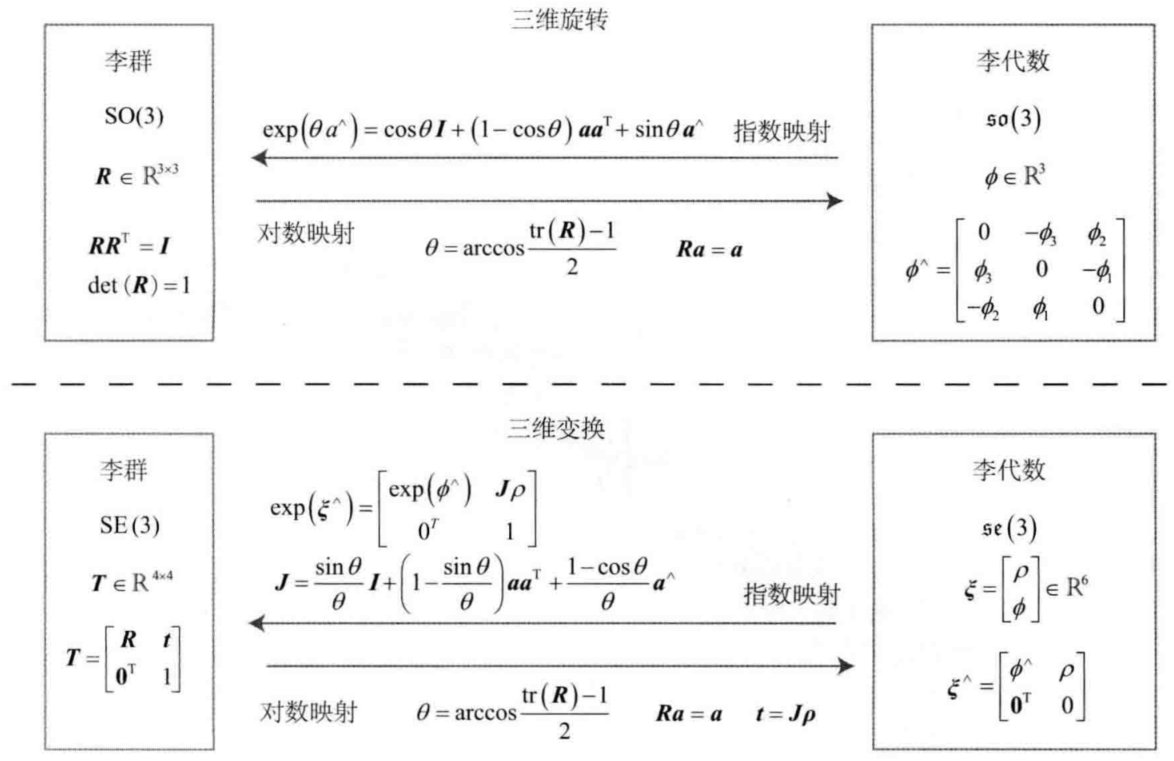
\includegraphics[width=\hsize]{images/对应关系.png}
    \caption{$SO(3),SE(3),\mathfrak{so}(3),\mathfrak{se}(3)$的对应关系} 
\end{figure}
\subsection{李代数求导与扰动模型}
使用李代数是为了进行优化,在优化过程中不可避免的有求导,那么李代数的求导如何进行?

李代数的指数映射与李群相对应,那么李代数的指数映射是否符合指数运算的基本规则,显然这是不成立的,因为$\exp{\phi\sphat}$中是
一个矩阵,不满足$\exp{(\phi_1\sphat)}\exp{(\phi_2\sphat)}=\exp{(\phi_1\sphat + \phi_2\sphat)}$,它满足的是一个
BCH公式(Baker-Campbell-Hausdorff),给出其完整公式的前面几项
\begin{align} 
    ln(\exp{(\mathbf{A})}\exp{(\mathbf{B})})=\mathbf{A}+\mathbf{B}+\frac{1}{2}[\mathbf{A},\mathbf{B}]+
    \frac{1}{12}[\mathbf{A},[\mathbf{A},\mathbf{B}]]-\frac{1}{12}[\mathbf{B},[\mathbf{A},\mathbf{B}]]+\cdot\cdot\cdot 
\end{align}
其中[]为李括号,当考虑$SO(3)$上的李代数$ln(\exp{(\phi_{1}\sphat)}\exp{(\phi_{2}\sphat)})\spcheck$,当$\phi_{1}$
或$\phi_{2}$为小两时,小量二次以上的项都可以被忽略,此时BCH拥有线性近似表达
\begin{align}
     ln(\exp{(\phi_{1}\sphat)}\exp{(\phi_{2}\sphat)})\spcheck\approx\left\{\begin{array}{l}\mathbf{J}_{l}
        (\phi_2)^{-1}\phi_{1}+\phi_{2}\quad\text{当$\phi_{1}$为小量} \\ \mathbf{J}_{r}(\phi_{1})^{-1}
        \phi_{2}+\phi_{1}\quad\text{当$\phi_{2}$为小量}\end{array}\right.
\end{align}
以上式的第一个近似为例,当对一个旋转矩阵$\mathbf{R}_{2}$(李代数为$\phi_{2}$)左乘一个微小旋转矩阵$\mathbf{R}_{1}$
(李代数为$\phi_{1}$)时,可以近似的看作,在原有李代数$\phi_{2}$上加了一项$\mathbf{J}_{l}(\phi_{2})\phi_{1}$,同理
第二个近似描述了右乘一个微小位移的情况。于是在BCH近似下,分成了左乘近似和右乘近似两种,以左乘为例
\begin{align} 
    \mathbf{J}_{l}=\mathbf{J}=\frac{\sin\theta}{\theta}\mathbf{I}+(1-\frac{\sin\theta}{\theta})\mathbf{a}
    \mathbf{a}^{T}+\frac{1-\cos\theta}{\theta}\mathbf{a}\sphat
\end{align}
它的逆为
\begin{align} 
    \mathbf{J}_{l}^{-1}=\frac{\theta}{2}\cot\frac{\theta}{2}\mathbf{I}+(1-\frac{\theta}{2}\cot\frac{\theta}{2})
    \mathbf{a}\mathbf{a}^{T}-\frac{\theta}{2}\mathbf{a}\sphat 
\end{align}
而右乘雅可比仅需对自变量取符号即可:
\begin{align} 
    \mathbf{J}_{r}(\phi)=\mathbf{J}_{l}(-\phi)
\end{align}

由此对某一旋转$\mathbf{R}$对应的李代数$\phi$给它左乘一个微小旋转$\Delta\mathbf{R}$(对应的李代数为$\Delta\phi$)
在李群上得到$\Delta\mathbf{R}\cdot\mathbf{R}$,而在李代数上,根据BCH相似,为$\mathbf{J}_{l}^{-1}(\phi)\Delta\phi
+\phi$,合并起来来可写为
\begin{align} 
    \exp{(\Delta\phi\sphat)}\exp{(\phi\sphat)}=\exp((\phi+\mathbf{J}_{l}^{-1}(\phi)\Delta\phi)\sphat)
\end{align} 
反之,在李代数上进行加法,让一个$\phi$加上$\Delta\phi$,那么可以近似为李群上带所有雅可比的乘法:
\begin{align} 
    \exp((\phi+\Delta\phi)\sphat)=\exp((\mathbf{J}_{l}\Delta\phi)\sphat)\exp(\phi\sphat)
    =\exp(\phi\sphat)\exp((\mathbf{J}_{r}\Delta\phi)\sphat)
\end{align}
同样对于$SE(3)$也有类似的BCH近似
\section{畸变和相机模型}
由透镜形状引起的畸变叫做径向畸变,会将现实中的一条直线变为一条曲线,它主要分为两大类\textbf{桶形畸变}和\textbf{枕形畸变},
桶形畸变图像放大率随着光轴之间的距离增加而减小,而枕行畸变恰好相反。在这两种畸变中穿过图像中心和光轴有交点的直线还能保持形状不变。
在相机的组装过程中不能使透镜和成像平面严格平行会引入\textbf{切向畸变}

归一化平面上任意一点$\mathbf{p}$坐标为$[x,y]^{T}$,也可用极坐标形式$[r,\theta]^{T}$,其中$r$表示点$\mathbf{p}$与坐标
系原点之间的距离,$\theta$表示与水平轴的夹角。径向畸变可以堪称坐标点沿着长度方向发生了变化,切向畸变可以看成坐标点沿着切线
方向发生了变化,对于径向畸变
\begin{align} 
    x_{distorted}=x(1+k_{1}r^{2}+k_{2}r^{4}+k_{3}r^{6}) \notag\\
    y_{distorted}=y(1+k_{1}r^{2}+k_{2}r^{4}+k_{3}r^{6})
\end{align} 
对于切向畸变可以用另外两个参数来表示
\begin{align} 
    x_{distorted}=x+2p_{1}xy+p_{2}(r^{2}+2x^{2}) \notag \\
    y_{distorted}=y+p_{1}(r^{2}+2y^{2})+2p_{2}xy
\end{align} 
联合上面的公式就可以通过五个畸变系数找到这个点在像素平面中正确的位置:
\begin{align} 
    \left\{\begin{array}{l}
        x_{distorted}=x(1+k_{1}r^{2}+k_{2}r^{4}+k_{3}r^{6})+x+2p_{1}xy+p_{2}(r^{2}+2x^{2}) \\
        y_{distorted}=y(1+k_{1}r^{2}+k_{2}r^{4}+k_{3}r^{6})+y+p_{1}(r^{2}+2y^{2})+2p_{2}xy
    \end{array}\right.
\end{align}
将畸变后的点通过内参数矩阵投影到像素平面,得到该点在图像上的正确位置:
\begin{align} 
    \left\{\begin{array}{l}
        u=f_{x}x_{distorted}+c_{x} \\
        v=f_{y}y_{distorted}+c_{y}
    \end{array}\right.
\end{align}
\section{极几何}
\textbf{三角化},已知两幅图片中对应真实世界中点$P$的两个像素坐标$p$和$p^{'}$,两个相机的内参$K$和$K^{'}$
以及两个相机之间的位姿变换矩阵$\mathbf{R}$和$\mathbf{T}$,求解$P$的三维坐标。即寻找$P$满足
\begin{align} 
    \left\{\begin{array}{l}p=MP=K[I\quad 0]P \\ p^{'}=M^{'}P=K^{'}[R\quad T]P\end{array}\right.
\end{align} 
但现实是对于相机内参$K$和$K^{'}$、相机位姿旋转矩阵$R$、平移向量$T$往往不知道,仅清楚两张图片之间的对应点
$p$和$p^{'}$。

于是在多视图几何中存在以下几个关键问题
\begin{enumerate}
    \item 摄像几何:从一张或者多张图像中求解摄像机的内外参数
    \item 场景几何:通过两张至多张图片寻找3D场景坐标
    \item 对应关系:已知一个图像中的$p$点,如何在另一个图像中找到对应的$p^{'}$点
\end{enumerate}
\begin{figure}[!htb]
    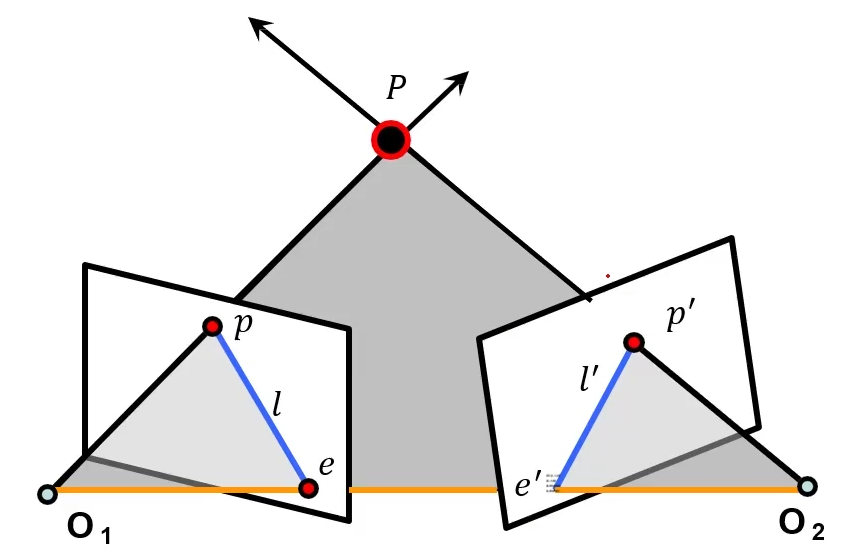
\includegraphics[width=\hsize]{images/极几何.png}
    \caption{极几何} 
\end{figure}
如图:
\begin{enumerate}
    \item 极平面:过点$P$,$O_{1}$与$O_{2}$的平面
    \item 基线:$O_{1}$与$O_{2}$的连线
    \item 极线:极平面与成像平面的交线
    \item 极点:基线与成像平面的交点
\end{enumerate}
极几何的特例:平行视图(常见双目立体、VR):
\begin{figure}[!htb]
    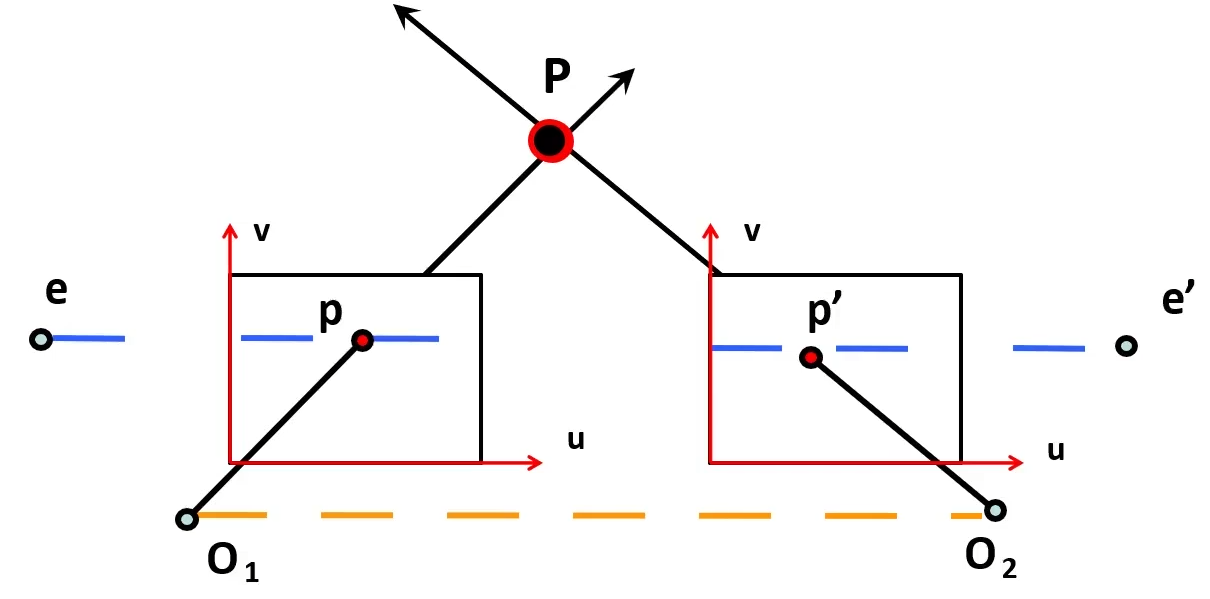
\includegraphics[width=\hsize]{images/平行视图.png}
    \caption{极几何的特例:平行视图} 
\end{figure}
\begin{enumerate}
    \item 两个图像平面平行
    \item 基线平行于图像平面,极点$e$和$e^{'}$位于无穷远处
    \item 极线平行于图像坐标系的$u$轴
\end{enumerate}
\subsection{本质矩阵}
对于规范化相机,图像$I$上点$p$像素坐标为$(u,v)$,图像$I^{'}$上的点$p^{'}$坐标为$(u^{'},v^{'})$,
$K=K^{'}=\left[\begin{array}{ccc}1&0&0\\0&1&0\\0&0&1\end{array}\right]$,因为为规范化相机
所以点$p$在$O_{1}$坐标系下的\textbf{非齐次坐标}为$(u,v,1)$,同理空间点$p^{'}$在$O_{2}$下的
\textbf{非齐次坐标}为$(u^{'},v^{'},1)$
知道$O_{1}$到$O_{2}$的旋转矩阵$R$和平移向量$T$,于是有
\begin{align} 
    &p^{'}\text{在}O_{1}\text{的坐标}=R^{T}p^{'}-R^{T}T \notag\\
    &O_{2}\text{在}O_{1}\text{的坐标}=-R^{T}T 
\end{align}
于是可以求得一个垂直于极平面的向量
\begin{align} 
    R^{T}T\times(R^{T}p^{'}-R^{T}T)=R^{T}T\times R^{T}p^{'}
\end{align}
因为$p$点在极平面上,所以有
\begin{align} 
    [R^{T}T\times R^{T}p^{'}]^{T}\cdot p=0
\end{align}
将上面的式子推导可以得出
\begin{align} 
    p^{'T}[T\times R]p=0 
\end{align}
于是点$p$和点$p^{'}$存在一个极几何约束-----本质矩阵
\begin{align} 
    &E=T\times R\Rightarrow E=\text{本质矩阵} \\
    &p^{'}Ep=0
\end{align}
其中本质矩阵有以下性质:
\begin{enumerate}
    \item $p$对应的极线是$l^{'}(l^{'}=Ep)$
    \item $p^{'}$对应的极线是$l(l=E^{T}p^{'})$
    \item $Ee=0$与$e^{'T}E=0$
    \item $E$是奇异的(秩2)
    \item $E$是5个自由度(三个旋转+三个平移,$det(E)$去掉一个自由度)
\end{enumerate}                
\subsection{基础矩阵}
这个为正常透视相机下的点$p$与点$p^{'}$的对应关系,此时推导类比规范化相机下的推导,先将两张图像上点的
坐标转换为规范化相机下的坐标,有:
\begin{align}
    \left\{\begin{array}{l}p_{c}=K^{-1}p\\p_{c}^{'}=K^{'-1}p^{'}\end{array}\right. 
\end{align}
于是有:$p_{c}^{'T}Ep_{c}=(K^{'-1}p^{'})^{T}\cdot[T_{\times}]RK^{-1}p=p^{'T}K^{'-T}
[T_{\times}]RK^{-1}p=0$
即可求得基础矩阵
\begin{align} 
    F=K^{'-T}[T_{\times}]RK^{-1}\rightarrow p^{'T}Fp=0
\end{align}
同样它也有上述的几个性质,不同的是它有7个自由度,因为尺度无法确定。

\noindent\textbf{常见的基础矩阵估计方法八点法,归一化八点法}
\subsection{单应性矩阵}
空间平面在两个摄像机下的投影几何
\begin{figure}[!htb]
    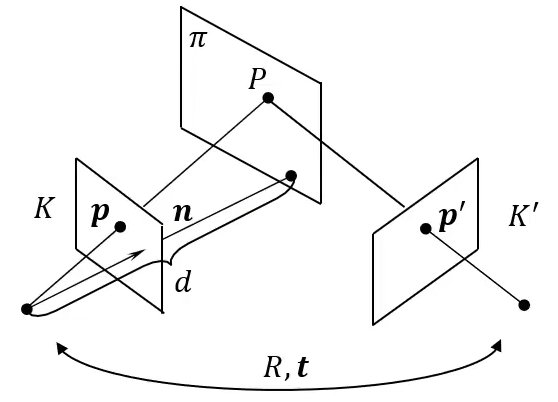
\includegraphics[width=\hsize]{images/单应性矩阵推导.png}
    \caption{单应性矩阵推导} 
\end{figure}
如图单应性矩阵推导已知第一个摄像机的内参矩阵$K$,第二个内参矩阵$K^{'}$,第二个摄像机相对于第一个摄像机
的位置$(R,t)$,$n$为平面$\pi$在第一个摄像机坐标系下的单位法向量,$d$为坐标原点到平面$\pi$的距离

平面$\pi$的方程为$n^{T}\tilde{P}=d$,$\tilde{P}$表示点$P$的欧式坐标,由此直接给出平面$\pi$的
单应性矩阵$H=K^{'}(R+tn_{d}^{T})K^{-1}$,其中,$n_{d}=\frac{n}{d}$

\textbf{约束关系}

基础矩阵建立点和极线的对应关系

单应矩阵建立点和点的对应







\newpage
\section{概率运动模型}
\subsection{速度运动模型}
理想模型,不考虑速度的误差机器人以速度$u_k$在很短时间$\Delta t$内做匀速运动,位姿从$x_{k-1}$转移到$x_k$。
\begin{figure}[!htb]
    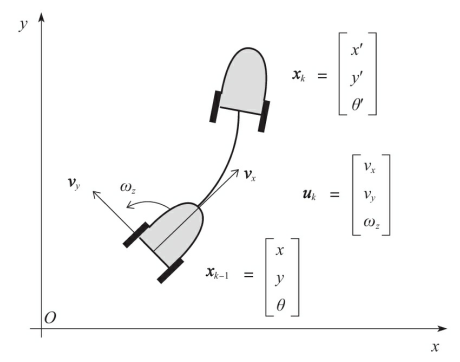
\includegraphics[width=\hsize]{images/速度运动模型.png}
    \caption{速度运动模型}
\end{figure}
\begin{align}  
    \mathbf{x}_{k}=\left[\begin{array}{c}x^{'} \\ y^{'} \\ \theta^{'} \end{array}\right]=
    g(\mathbf{x}_{k-1},\mathbf{u}_{K}) = \left[\begin{array}{c} x \\ y \\ \theta\end{array}\right]
    +\left[\begin{array}{ccc} \cos{\theta} & -\sin{\theta} & 0 \\ \sin{\theta} & \cos{\theta}
    & 0 \\ 0 & 0 & 1 \\ \end{array}\right] \left[\begin{array}{c}v_x \\ v_y \\ \omega_{z} 
    \end{array}\right] \Delta t
\end{align}

考虑速度的误差,在实际中,需要考虑$u_{k}、x_{k-1}、x_{k}$的误差,这里简单假设为服从高斯分布
\begin{align} 
    &\mathbf{u} \backsim N(\overline{\mathbf{u}}_{k},\Sigma_{\mathbf{u}_{k}}) \notag\\
    &\mathbf{x}_{k-1} \backsim N(\overline{\mathbf{x}}_{k-1},\Sigma_{\mathbf{x}}) \\
    &\mathbf{x}_{k} \backsim N(\overline{\mathbf{x}}_{k},\Sigma_{\mathbf{x}_{k}}) \notag
\end{align}
这样,$u_{k}、x_{k-1}、x_{k}$都变成了多元随机变量,随机变量的均值就是其估计值,用协方差矩阵描述其不确定性大小。
$u_{k}$的误差主要是由3个速度分量$v_{k}、v_{y}、\omega_{z}$的误差决定的,所以$u_{k}$的协方差矩阵如下所示
\begin{align} 
    \Sigma_{\mathbf{u}_{k}}=\left[\begin{array}{ccc}\sigma_{v_{x}}^{2} & 0 & 0 \\
        0 & \sigma_{v_{y}}^{2} & 0 \\ 0 & 0 & \sigma_{\omega_{z}}^{2}\end{array}\right]  
    \end{align}
已知$u_{k}$和$x_{k-1}$的分布特性,利用运动的状态转移公式就可以推导出$x_{k}$的分布特性,即状态转移概率
$\mathbf{P}(\mathbf{x}_k|\mathbf{x}_{k-1},\mathbf{u}_k)$。其中一个最简单的方法是先将状态转移函数g
进行一阶泰勒级数展开来实现线性化,然后直接通过线性计算就能够得到$x_{k}$的协方差矩阵
\begin{align}
    \Sigma_{x_{k}}=\left[\begin{array}{cc}\frac{\partial g}{\partial \mathbf{x}_{k-1}} & 
        \frac{\partial g}{\partial \mathbf{u}_k}\end{array}\right]
        \left[\begin{array}{cc}\Sigma_{x_{k-1}} & \mathbf{0}_{3 \times 3}\\
            \mathbf{0}_{3\times 3} & \Sigma_{\mathbf{u}_k}\end{array}\right]
        \left[\begin{array}{cc}\frac{\partial g}{\partial \mathbf{x}_{k-1}} & 
        \frac{\partial g}{\partial \mathbf{u}_k}\end{array}\right]^{T}
\end{align} 
其中,$\left[\begin{array}{cc}\frac{\partial g}{\partial \mathbf{x}_{k-1}} & \frac{\partial g}{\partial \mathbf{u}_k}\end{array}\right]$
为函数$g$的雅可比矩阵。
上面的推导都是基于两大假设,一是运动时间$\Delta t$很小,二是$u_k、x_{k-1}、x_{k}$的误差都服从高斯分布。
\subsection{里程计运动模型}
上面的速度运动模型中有太强的假设,准确性很难保证,实际中机器人一般配备有里程计等感知传感器来用于反馈运动。
通过前后两个里程计的差值,可以求出里程计的增量值$u_{K}$,即所谓的机器人状态转移量。
\begin{align}  
    \mathbf{u}_{k}=\textbf{odom}_k - \textbf{odom}_{k-1}=
    \left[\begin{array}{c}\Delta x \\ \Delta y \\ \Delta \theta\end{array}\right] 
\end{align}
与讨论速度运动模型一样,先不讨论有误差的模型,直接推导状态转移概率$\mathbf{P}(\mathbf{x}_k|
\mathbf{x}_{k-1},\mathbf{u}_k)$的数学形式。
\begin{figure}[!htb]
    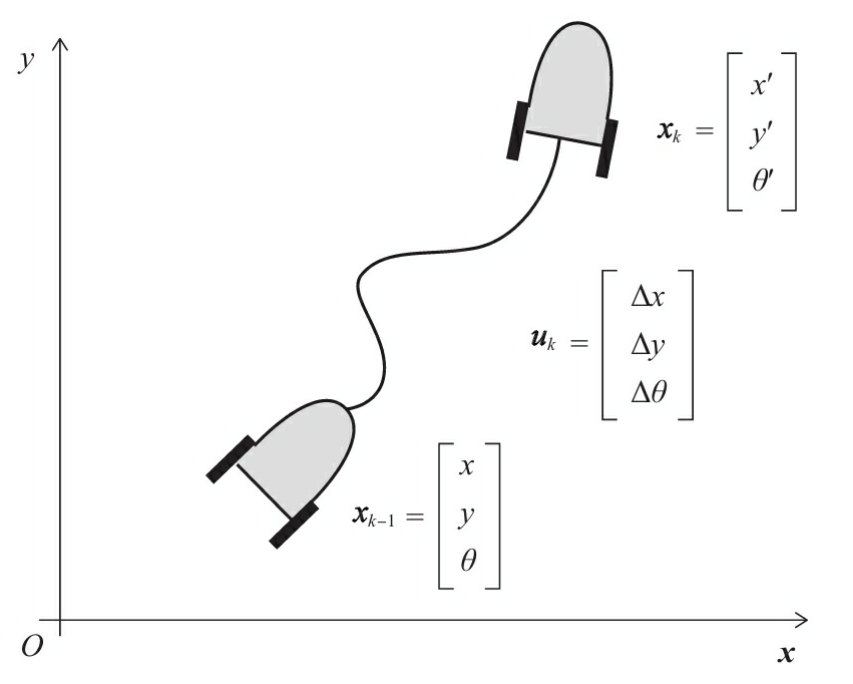
\includegraphics[width=\hsize]{images/里程计运动模型.png}
    \caption{里程计运动模型} 
\end{figure}    
此时可直接求出$x_k$
\begin{align}  
    \mathbf{x}_{k}=\left[\begin{array}{c}x^{'} \\ y^{'} \\ \theta^{'}\end{array}\right]
    =g(\mathbf{x}_{k-1},\mathbf{u}_{k})=\left[\begin{array}{c}x \\ y \\ \theta \end{array}\right] 
    +\left[\begin{array}{c}\Delta x \\ \Delta y \\ \Delta \theta \end{array}\right]
\end{align}

考虑历程计误差的情况下,这里将$u_k$通用的表示在三维空间运动,但是机器人底盘被限制在二维平面运动,所以其中z轴的偏移量、
x轴的旋转量和y轴的旋转量均为0。
\begin{align} 
    \Sigma_{u_k}=\left[\begin{array}{cccccc}
        \sigma_{\Delta x}^{2} & 0 & 0 & 0 & 0 & 0 \\
        0 & \sigma_{\Delta y}^{2} & 0 & 0 & 0 & 0 \\
        0 & 0 & 0 & 0 & 0 & 0 \\
        0 & 0 & 0 & 0 & 0 & 0 \\
        0 & 0 & 0 & 0 & 0 & 0 \\
        0 & 0 & 0 & 0 & 0 & \sigma_{\Delta\theta}^{2} \\
    \end{array}\right]
\end{align}

轮式里程计是存在累计误差的,即机器人地盘运动得越远累积误差越大。可以用运动距离$\sqrt{(\Delta x)^{2}+(\Delta y)^{2}}$
和旋转量$|\Delta \theta|$来量化$u_k$的误差。
\begin{align} 
    &\sigma_{\Delta x}^{2}=\xi_{\Delta xy}+\alpha_{1}\sqrt{(\Delta x)^{2}+(\Delta y)^{2}} + \alpha_{2}|\Delta \theta| \notag \\
    &\sigma_{\Delta y}^{2}=\xi_{\Delta xy}+\alpha_{1}\sqrt{(\Delta x)^{2}+(\Delta y)^{2}} + \alpha_{2}|\Delta \theta| \\
    &\sigma_{\Delta \theta}^{2}=\xi_{\Delta \theta}+\alpha_{3}\sqrt{(\Delta x)^{2}+(\Delta y)^{2}} + \alpha_{4}|\Delta \theta| \notag
\end{align}    
\section{概率观测模型} 
这先介绍激光模型
\subsection{波束模型}
每个激光束可以得到一个距离值$z_{k}^{i}$,对于$n$个测量值$\mathbf{z}_{k}=\{z_{k}^{1},z_{k}^{2},...,z_{k}^{n}\}$,
那么观测$z_k$的不确定性由每个单独光束测量值的不确定性相乘得到
\begin{align} 
    P(\mathbf{z}_k | \mathbf{x}_k,\mathbf{m})=\prod_{i=1}^{n}P(z_{k}^{i} | \mathbf{x}_k,\mathbf{m})
\end{align} 
根据实验和经验所得,单个激光束测距值误差主要分为四类:读书误差、动态干扰、测量失效和随机误差。

读数误差,传感器由于构造、计算精度、分辨率等因素给测量带来的误差,可直接用高斯分布来表示,其中$\eta_{hit}$是归一化
因子,$z_{max}$是激光束的最大测量值。
\begin{align}  
    P(z_{k}^{i} | \mathbf{x}_k,\mathbf{m}) =\left\{\begin{array}{l}\eta_{hit}N(\overline{z}_{k}^{i},
    \sigma_{hit}^{2}),0\leq z_{k}^{i} \leq z_{max} \\ 0, \text{其它} \end{array}\right.
\end{align}

动态干扰误差,环境中动态障碍物挡住激光束,导致原本对应在地图中的障碍物的测量距离变短,采用指数分布来表示,其中$\eta_{short}$
是归一化因子,$\lambda_{short}$是指数分布参数
\begin{align} 
    P_{short}(z_{k}^{i} | \mathbf{x}_k, \mathbf{m}) = \left\{\begin{array}{l}\eta_{short}\lambda_{short}
    \exp^{-\lambda_{short}z_{k}^{i}},0\leq z_{k}^{i}\leq \overline{z}_{k}^{i} \\ 0,\text{其它}\end{array}
    \right. 
\end{align}

环境中的黑色吸光、透明、镜面反反射等障碍物会导致测量失效,使得激光测距值超量程或者无穷远,这用最大量程$z_{max}$附近的
窄矩形分布来描述
\begin{align}  
    P_{max}(z_{k}^{i} | \mathbf{x}_k,\mathbf{m})=\left\{\begin{array}{l}\frac{1}{\varepsilon},z_{max}
    -\varepsilon \leq z_{k}^{i} \leq z_{max} \\ 0,\text{其它} \end{array}\right.
\end{align}

最后哪些不能明确建模的误差,用一个均匀分布的随机误差来统一描述,均匀分布的范围是整个量程区间
\begin{align} 
    P_{rand}(z_{k}^{i} | \mathbf{x}_{k},\mathbf{m})=\left\{\begin{array}{l}\frac{1}{z_{max}},0\leq 
    z_{k}^{i} \leq z_{max} \\ 0,\text{其它}\end{array}\right.
\end{align}

将上述四种误差加权平均后就是光束模型,其中$z_{hit},z_{short},z_{max},z_{rand}$为加权系数,它们的和为1,加权后的
概率分布为
\begin{align} 
    P(z_{k}^{i} | \mathbf{x}_{k},\mathbf{m}) = z_{hit}\cdot P_{hit}+z_{short}\cdot P_{short}+
    z_{max}\cdot P_{max}+z_{rand}\cdot P_{rand}
\end{align}
\begin{figure}[!htb]
    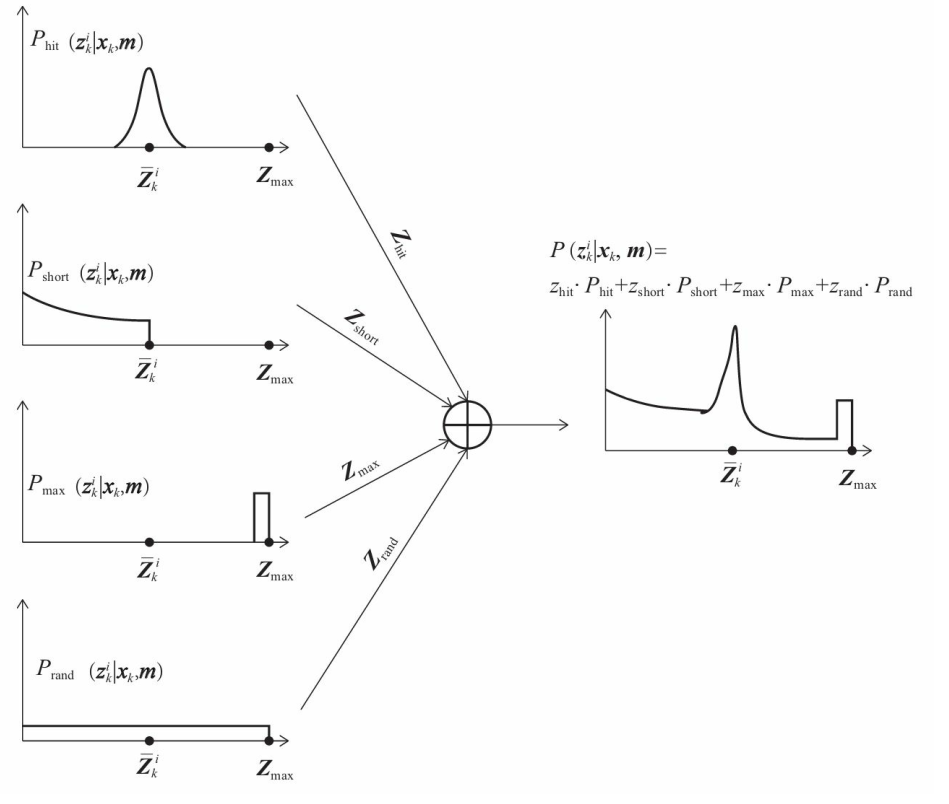
\includegraphics[width=\hsize]{images/波束模型的概率描述.png}
    \caption{波束模型的概率描述}
\end{figure}
\subsection{似然域模型}
它的思路是利用测量值对应的机器人位姿,将测量值$z_{k}^{i}$透射到已有的地图上,将超过量程的测量值直接丢弃,然后用似然域
描述测量值分布。所谓似然域就是激光束上障碍物出现的概率大小由其附近的地图点远近决定。
\subsection{概率图模型}












\end{document}